\expandafter\let\csname ver@amssymb.sty\endcsname\empty
\documentclass[serif]{beamer}
\expandafter\let\csname ver@amssymb.sty\endcsname\relax
\usepackage{etex}
\usepackage[bitstream-charter]{mathdesign} % Use BT Charter font
\usepackage[T1]{fontenc}                   % Use T1 encoding instead of OT1
\usepackage[utf8]{inputenc}                % Use UTF8 input encoding
\usepackage{microtype}                     % Improve typography
\usepackage{booktabs}
\usepackage{cancel}
\usepackage{algorithm}
\usepackage{algorithmicx}
\usepackage{algpseudocode}
\usepackage{hyperref}
\hypersetup{pdfstartview=Fit}
\usepackage{tikz}
\usetikzlibrary{shapes,snakes,shadows,arrows,calc}
\usepackage{multirow}
\usepackage{animate}
\usepackage{moresize}
\usepackage{colortbl}
\usepackage{xcolor}
\usepackage{amsmath}
\usepackage{etoolbox}
\usepackage{listings}

\renewcommand\footnotemark{}

\lstset{
  columns=fullflexible,
  showspaces=false,
  showtabs=false,
  showstringspaces=false,
  commentstyle=\color{gray}\upshape,
}
\lstset{language=bash,frame=single,basicstyle=\ttfamily\footnotesize}
\lstdefinelanguage{XML}
{
  basicstyle=\ttfamily\scriptsize,
  morestring=[b]",
  frame=single,
  backgroundcolor=\color{gray!20},
% morestring=[s]{>}{<},
  morecomment=[s]{<?}{?>},
  morecomment=[s]{<!--}{-->},
  stringstyle=\color{red},
  identifierstyle=\color{darkblue},
  keywordstyle=\color{cyan},
}

\definecolor{gray}{rgb}{0.4,0.4,0.4}
\definecolor{darkblue}{rgb}{0.0,0.0,0.6}
\definecolor{cyan}{rgb}{0.0,0.6,0.6}

\usetheme{Copenhagen}
\usecolortheme{beaver}

\title{OpenMC Module: Description of OpenMC}
\author{\emph{Computational Reactor Physics Group}}
\date{\normalsize Department of Nuclear Science and Engineering\\
                  Massachusetts Institute of Technology}
% Set Logo
\logo{
\includegraphics[scale=0.2]{src/crpg.png}\hspace*{8cm}

\includegraphics[scale=0.2,trim=0cm 3.0cm 2.2cm 0cm, clip=true]{src/mitlogo.pdf}}

\usenavigationsymbolstemplate{}

%-------------------------------------------------------------------------------
\begin{document}
%-------------------------------------------------------------------------------

\frame{\titlepage}\logo{} % remove logo after title page

%-------------------------------------------------------------------------------

\begin{frame}{Goals of the OpenMC Project}
  \begin{itemize}
    \vfill
    \item<1-> Develop a Monte Carlo framework for reactor analysis that scales
      on leadership-class supercomputers (100,000+ cores)
    \vfill
    \item<1-> Provide a simple tool to analyze performance and limitations on
      proposed architectures
    \vfill
    \item<1-> Objectives:
      \begin{itemize}
      \item<1-> Realistic physics
      \item<1-> Modern programming style and data structures
      \item<1-> Extensible for research purposes
      \item<1-> Open source and freely available
      \vfill
      \end{itemize}
  \end{itemize}
\end{frame}

%-------------------------------------------------------------------------------

\begin{frame}{Characteristics of OpenMC}
  \begin{itemize}
  \item<1-> Fixed source and $k$-eigenvalue calculations
  \item<1-> Geometry: constructive solid geometry, second-order surfaces
    \begin{itemize}
    \item<1-> Universes and lattices
    \item<1-> Rotations and translations
    \end{itemize}
  \item<1-> Cross sections: ACE format (MCNP, Serpent)
  \item<1-> Physics: Only neutrons for now
    \begin{itemize}
    \item<1-> $S(\alpha,\beta)$ thermal scattering
    \item<1-> Unresolved resonance probability tables
    \item<1-> Free gas thermal scattering
    \end{itemize}
  \item<1-> Plotting: rasterization using find\_cell
  \item<1-> Tallies:
    \begin{itemize}
    \item<1-> Collision and path-length estimators
    \item<1-> Surface and volume mesh tallies
    \end{itemize}
  \item<1-> Distributed memory parallelism via MPI
  \item<1-> XML input format, HDF5 output format
  \end{itemize}
\end{frame}

%-------------------------------------------------------------------------------

\begin{frame}{Parallel Performance}
  \begin{columns}
    \column<1->{0.35\textwidth}
    \begin{center}
      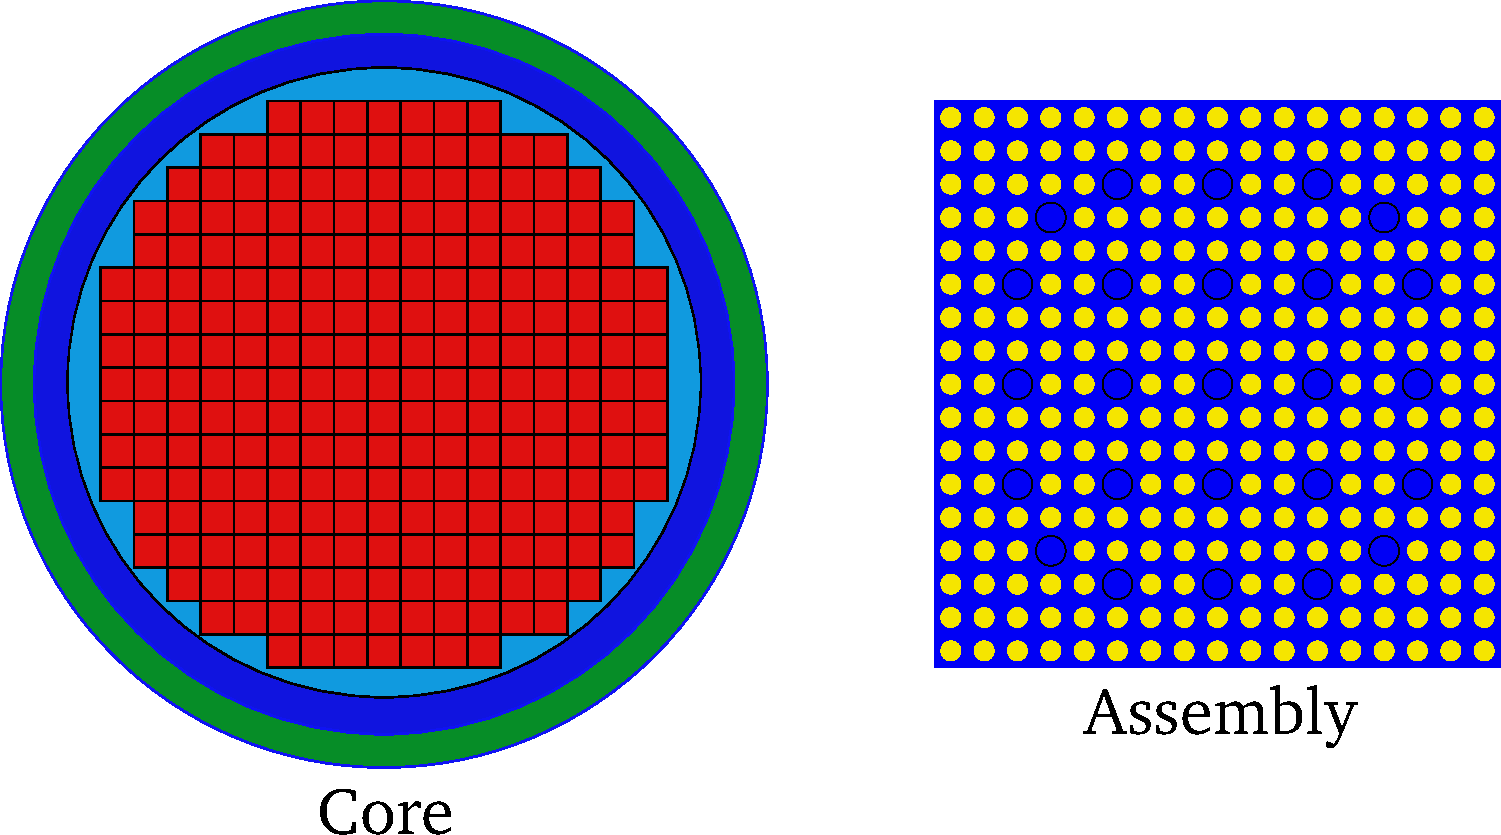
\includegraphics[width=1.7in]{src/mcperformance.pdf}
    \end{center}
    \footnotesize{
      \begin{itemize}
      \item<1-> $2^{17} = 131,072$
      \item<1-> Cray XK6 = ORNL Jaguar
      \item<1-> Blue Gene/P = ANL Intrepid
      \end{itemize}
    }
    \column<1->{0.65\textwidth}
    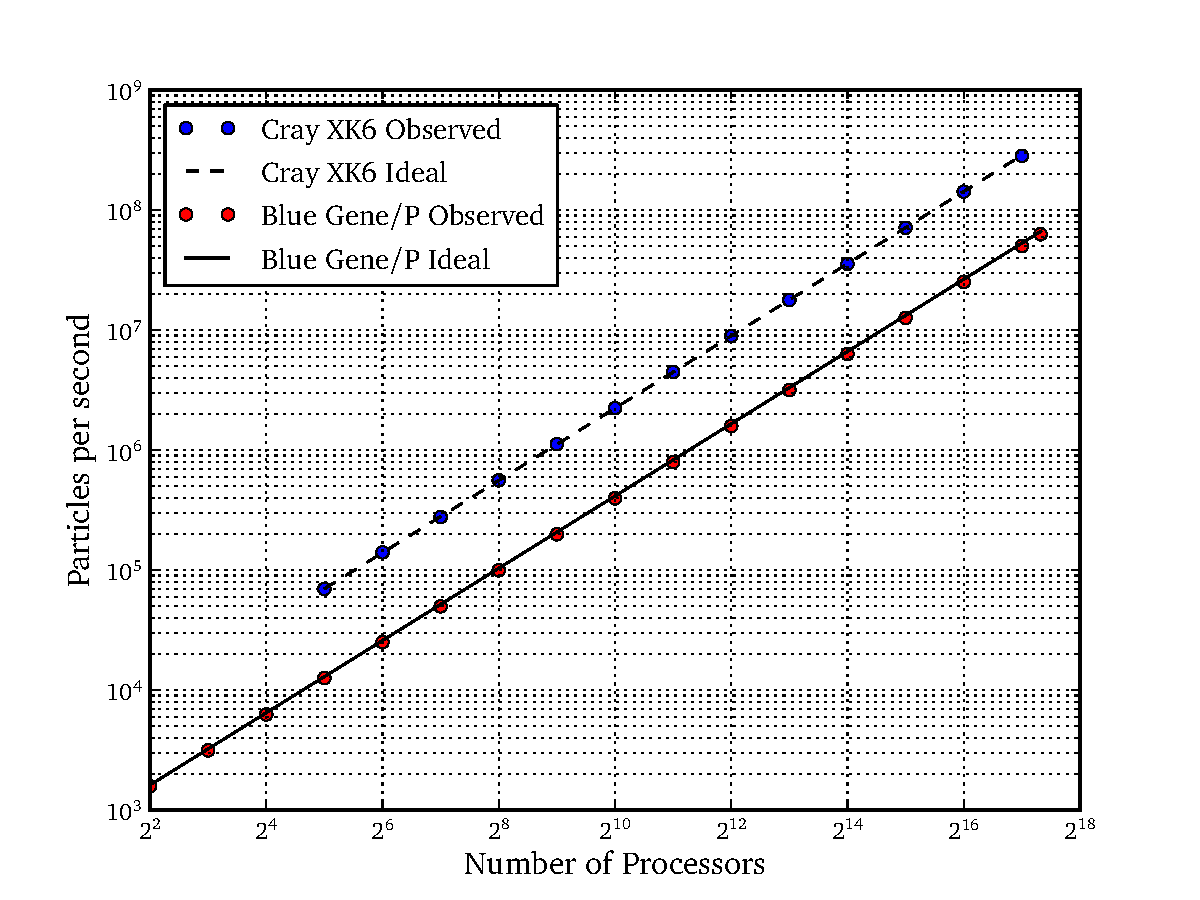
\includegraphics[width=3.0in]{src/scaling_loglog.pdf}
  \end{columns}
\end{frame}

%-------------------------------------------------------------------------------

\begin{frame}{Validation and Verification}
  \begin{itemize}
  \item<1-> MCNP Criticality Benchmark Suite
    \begin{itemize}
    \item<1-> 119 configurations --- different spectra, materials, enrichment
    \item<1-> Models built for all but two
    \end{itemize}
  \end{itemize}
  \centerline{
    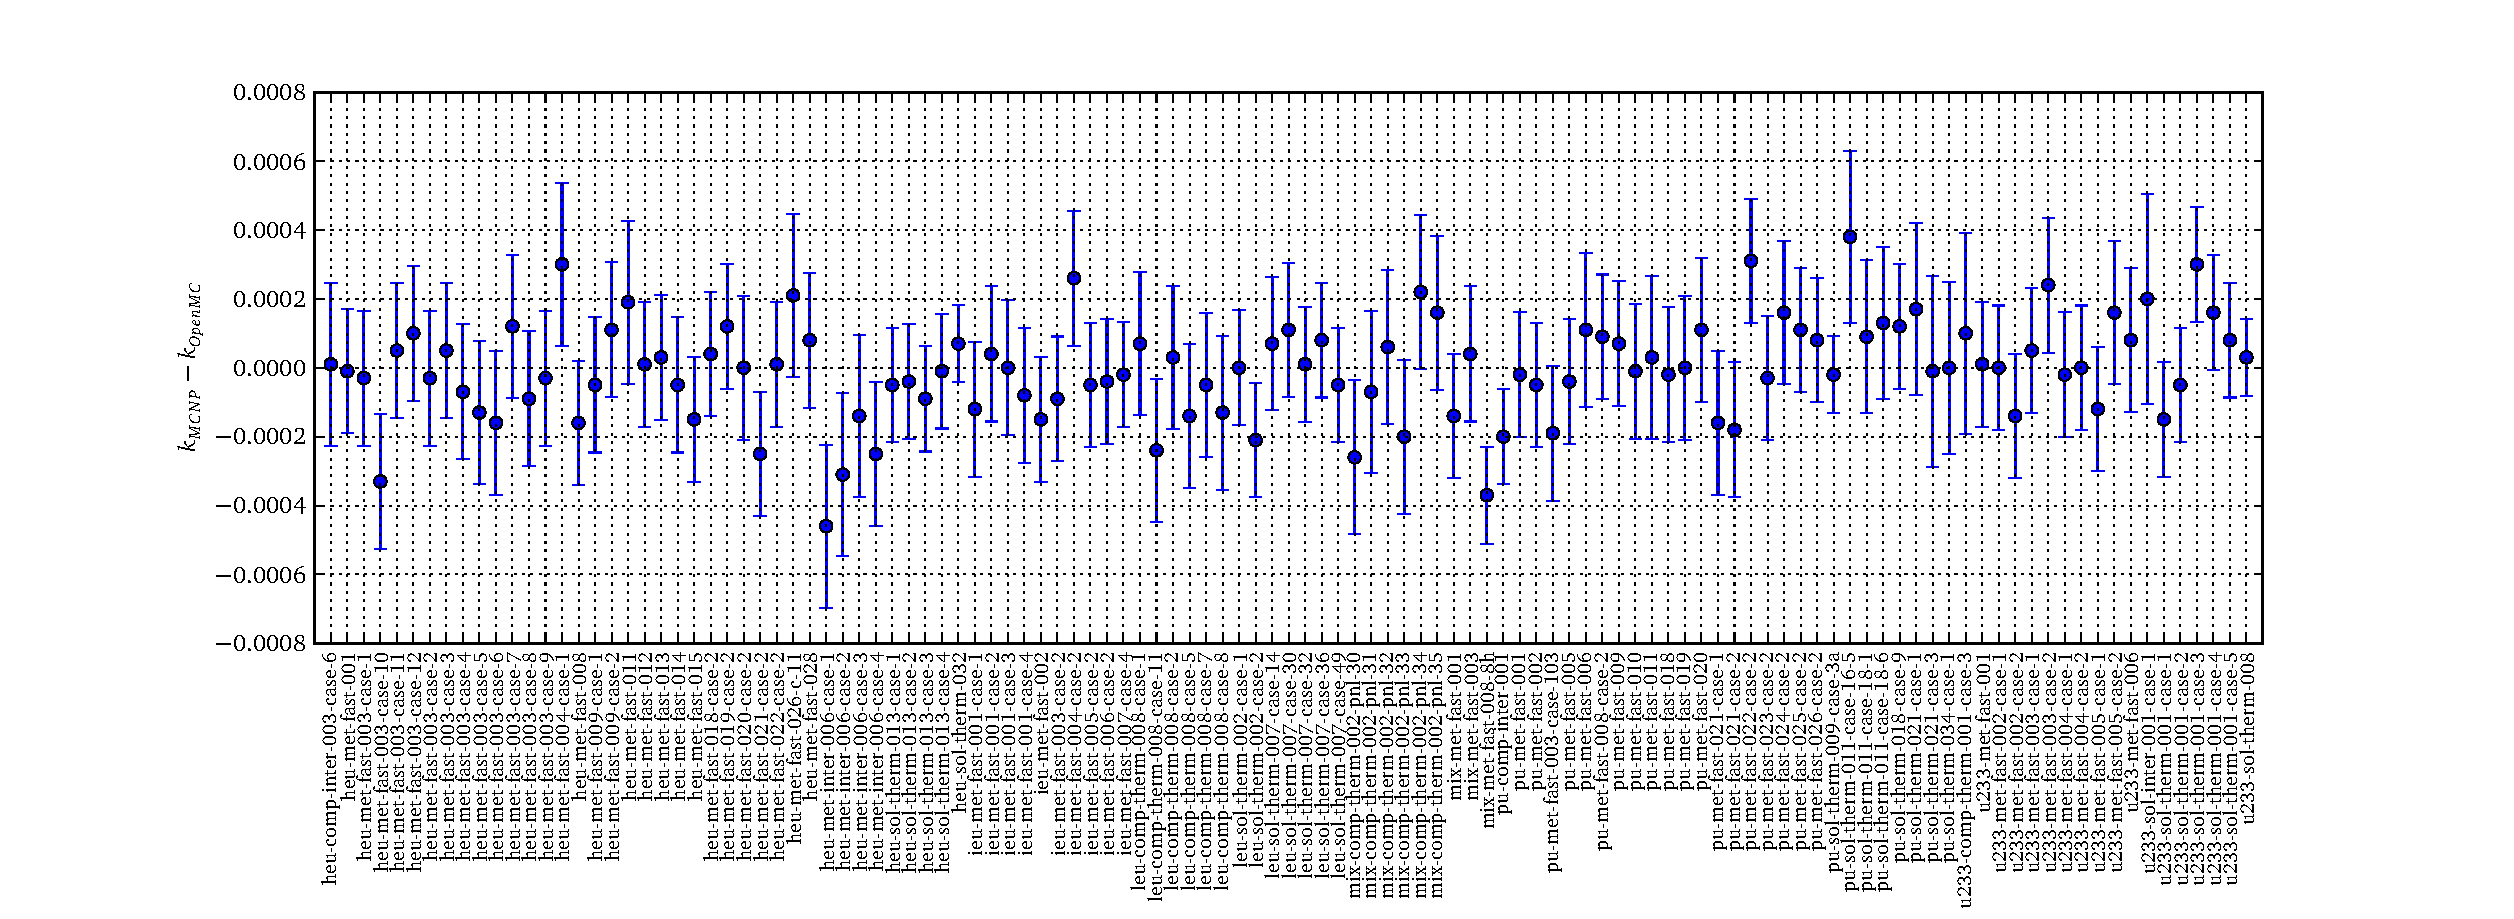
\includegraphics[width=1.35\textwidth]{src/expanded-suite.pdf}
  }
\end{frame}

%-------------------------------------------------------------------------------

\begin{frame}{MIT/X License}
  \footnotesize{
  \begin{itemize}
  \item<1-> Permission is hereby granted, free of charge, to any person
    obtaining a copy of this software and associated documentation files (the
    “Software”), to deal in the Software without restriction, including
    without limitation the rights to use, copy, modify, merge, publish,
    distribute, sublicense, and/or sell copies of the Software, and to permit
    persons to whom the Software is furnished to do so, subject to the following
    conditions:
  \item<1-> The above copyright notice and this permission notice shall be
    included in all copies or substantial portions of the Software.
  \item<1-> THE SOFTWARE IS PROVIDED “AS IS”, WITHOUT WARRANTY OF ANY KIND,
    EXPRESS OR IMPLIED, INCLUDING BUT NOT LIMITED TO THE WARRANTIES OF
    MERCHANTABILITY, FITNESS FOR A PARTICULAR PURPOSE AND NONINFRINGEMENT. IN NO
    EVENT SHALL THE AUTHORS OR COPYRIGHT HOLDERS BE LIABLE FOR ANY CLAIM,
    DAMAGES OR OTHER LIABILITY, WHETHER IN AN ACTION OF CONTRACT, TORT OR
    OTHERWISE, ARISING FROM, OUT OF OR IN CONNECTION WITH THE SOFTWARE OR THE
    USE OR OTHER DEALINGS IN THE SOFTWARE.
  \end{itemize}
  }
\end{frame}

% -----------------------------------------------------------------------------

\begin{frame}[fragile]{Obtaining OpenMC}
  \begin{itemize}
  \vfill
  \item<1-> Online at \url{https://github.com/mit-crpg/openmc}
  \vfill
  \item<1-> git:
\begin{lstlisting}
git clone git://github.com/mit-crpg/openmc.git
\end{lstlisting}
  \vfill
  \item<1-> Ubuntu PPA:
\begin{lstlisting}
sudo apt-add-repository ppa:paulromano/staging
sudo apt-get update
sudo apt-get install openmc
\end{lstlisting}
  \vfill
  \end{itemize}
\end{frame}

%-------------------------------------------------------------------------------

\begin{frame}[fragile]{Compiling on Linux/Mac OS X}
  \begin{itemize}
  \vfill
  \item<1-> $\sim$30,000 lines of Fortran 2008 code
  \vfill
  \item<1-> All handled by a Makefile
\begin{lstlisting}
cd openmc/src
make
sudo make install
\end{lstlisting}
  \vfill
  \item<1-> Optional dependencies
    \begin{itemize}
    \item<1-> MPI for distributed-memory parallelism
    \item<1-> HDF5 for portable standard binary output format
    \item<1-> PETSc for CMFD acceleration
    \end{itemize}
  \vfill
  \item<1-> Works with gfortran, Intel, IBM, Cray, PGI compilers
  \vfill
  \item<1-> On Mac OS X, can obtain compiler via Mac Ports
  \vfill
  \end{itemize}
\end{frame}

%-------------------------------------------------------------------------------

\begin{frame}{Compiling on Windows}
  \begin{itemize}
  \item<1-> Uninstall Windows
  \item<1-> Install a better operating system, like Linux
  \item<1-> Follow previous directions
  \end{itemize}
\end{frame}

%-------------------------------------------------------------------------------

\begin{frame}{Compiling on Windows}
  \begin{itemize}
  \vfill
  \item<1-> No native Windows binaries (yet)
  \vfill
  \item<1-> Options: Cygwin or MinGW (Minimalist GNU for Windows)
  \vfill
  \item<1-> Successful builds using both
  \vfill
  \item<1-> Visual Studio Port:
    \url{https://bitbucket.org/Lockee/openmc\_vs2010}
  \vfill
  \end{itemize}
\end{frame}

%-------------------------------------------------------------------------------

\begin{frame}{Cross Sections}
  \begin{itemize}
  \item<1-> You'll need:
    \begin{itemize}
    \vfill
    \item<1-> A set of ACE format cross sections
    \vfill
    \item<1-> A cross\_sections.xml file
    \vfill
    \end{itemize}
  \vfill
  \item<1-> Cross section data is not currently distributed with the code. Your
    options are:
    \begin{itemize}
    \vfill
    \item<1-> Obtain JEFF data in ACE format from OECD/NEA
    \vfill
    \item<1-> Use data from MCNP or Serpent
    \vfill
    \item<1-> Process raw ENDF/B data into ACE format using NJOY
    \vfill
    \end{itemize}
  \end{itemize}
\end{frame}

%-------------------------------------------------------------------------------

\begin{frame}{XML Input Format}
  \begin{itemize}
  \item<1-> Unlike many nuclear codes, OpenMC uses a modular XML input format
    \begin{itemize}
    \vfill
    \item<1-> Building a geometric model --- \textbf{geometry.xml}
    \vfill
    \item<1-> Define materials in problem --- \textbf{materials.xml}
    \vfill
    \item<1-> Settings paramters for the simulation --- \textbf{settings.xml}
    \vfill
    \item<1-> Determining which quantities to score --- \textbf{tallies.xml}
    \vfill
    \item<1-> Creating geometry plots --- \textbf{plots.xml}
    \vfill
    \item<1-> Setting CMFD parameters --- \textbf{cmfd.xml}
    \vfill
    \end{itemize}
  \end{itemize}
\end{frame}

%-------------------------------------------------------------------------------

\begin{frame}{XML Basics}
  \begin{itemize}
  \item<1-> XML = e\textbf{X}tensible \textbf{M}arkup \textbf{L}anguage
  \item<1-> Two kinds of information in a file:
    \begin{itemize}
    \item<1-> \textit{Markup}, like \texttt{<firstName>}, that describes the
      structure of the document, and
    \item<1-> \textit{Text}, like ``Paul'', that is the actual content of the document
    \end{itemize}
  \item<1-> All text must be contained within \textit{opening} and
    \textit{closing} tags, e.g. \texttt{<firstName>Paul</firstName>}
  \end{itemize}
\end{frame}

%-------------------------------------------------------------------------------

\begin{frame}[fragile]{XML Basics}
  \begin{itemize}
  \item<1-> Nesting of elements usually represents logical relationships:
    \begin{lstlisting}[language=XML]
<?xml version="1.0"?>
<EmployeeDatabase>

  <!-- Information about our employees -->

  <employee>
    <firstName>Paul</firstName>
    <lastName>Romano</lastName>
    <age>26</age>
  </employee>

  <employee firstName="Li" lastName="Zhu" age="34" />

</EmployeeDatabase>
    \end{lstlisting}
  \end{itemize}
\end{frame}

%-------------------------------------------------------------------------------

\begin{frame}{Running a simulation}
  \begin{itemize}
  \item<1-> Executable compiled
  \item<1-> Directory with XML files
  \item<1-> \texttt{openmc [/path/to/directory]}
  \end{itemize}
\end{frame}

%-------------------------------------------------------------------------------

\begin{frame}{Online documentation}
  \begin{itemize}
  \item<1-> When in doubt, check the user's guide!
  \item<1-> \url{http://mit-crpg.github.com/openmc}
  \end{itemize}
\end{frame}

%-------------------------------------------------------------------------------
\end{document}
%-------------------------------------------------------------------------------
